% ESR of DPPH and MnCl2 -- lab report, ETH physics lab, measurement 23 October 2026
% Build: make   (figures and appendix table: make figures, runs the analysis in ../analysis)
\documentclass[a4paper,11pt,DIV=12,abstract=true,numbers=noenddot]{scrartcl}

\usepackage[T1]{fontenc}
\usepackage{lmodern}
\usepackage[american]{babel}
\usepackage[autostyle]{csquotes}
\usepackage{microtype}
\usepackage{amsmath,amssymb}
\usepackage[locale=US, uncertainty-mode=separate, per-mode=symbol, range-phrase={\,\text{--}\,}, range-units=single, group-digits=integer]{siunitx}
\DeclareSIUnit{\angstrom}{\text{\AA}}
\usepackage[version=4]{mhchem}
\usepackage{graphicx}
\usepackage{booktabs}
\usepackage{tabularx}
\usepackage{xcolor}
\usepackage{tikz}
\usetikzlibrary{arrows.meta,positioning,calc}
\usepackage[font=small,labelfont=bf,format=plain]{caption}
\usepackage{enumitem}
\usepackage[hidelinks]{hyperref}
\usepackage{cleveref}
\crefname{figure}{Fig.}{Figs.}
\Crefname{figure}{Fig.}{Figs.}
\crefname{table}{Table}{Tables}
\Crefname{table}{Table}{Tables}
\crefname{equation}{Eq.}{Eqs.}
\Crefname{equation}{Eq.}{Eqs.}
\crefname{section}{Section}{Sections}
\Crefname{section}{Section}{Sections}
\crefname{subsection}{Section}{Sections}
\Crefname{subsection}{Section}{Sections}
\crefname{appendix}{Appendix}{Appendices}
\Crefname{appendix}{Appendix}{Appendices}

\setlist{nosep, leftmargin=*}
\setkomafont{disposition}{\normalcolor\bfseries}
\setcapindent{0pt}
\addtokomafont{caption}{\small}
\setlength{\abovecaptionskip}{4pt}

% ---------------------------------------------------------------- Macros
\newcommand*{\dd}{\mathrm{d}}
\newcommand*{\ii}{\mathrm{i}}
\newcommand*{\muB}{\mu_\mathrm{B}}
\newcommand*{\kB}{k_\mathrm{B}}
\newcommand*{\Bpp}{\Delta B_\mathrm{pp}}
\newcommand*{\Bhalf}{\Delta B_{1/2}}
\newcommand*{\Br}{B_\mathrm{r}}
\newcommand*{\Bm}{B_\mathrm{m}}
\newcommand*{\QL}{Q_\mathrm{L}}
\newcommand*{\lamg}{\lambda_\mathrm{g}}
\newcommand*{\chiI}{\chi'}
\newcommand*{\chiII}{\chi''}
% keep the space around binary operators (including the \pm of siunitx) from shrinking to zero in tight lines
\AtBeginDocument{\medmuskip=4mu plus 2mu minus 1mu}
\newenvironment{exercise}[1]{\par\smallskip\noindent$\blacktriangleright$\,\textbf{Preparatory exercise #1.}\ }{\par\smallskip}

\subject{Physics Laboratory III \textperiodcentered{} ETH Zürich}
\title{Electron Spin Resonance of DPPH and \ce{MnCl2}}
\author{Janosch Krauss}
\date{Measured on 23~October 2026 \textperiodcentered{} Report of 31~October 2026}

\begin{document}
\maketitle

% ====================================================================
\begin{abstract}
\noindent
I measured the electron spin resonance (ESR) of DPPH and \ce{MnCl2} with an X-band reflection spectrometer
(\qty{9.36}{GHz}). At the sample position the magnet's Hall probe reads too low, by \qty{8.5}{\percent} on the
analog output and \qty{2.3}{\percent} on the display, so I calibrated the field scale with the precisely known $g$-factor
of DPPH. The DPPH line has the peak-to-peak width $\Bpp=\qty{0.240(15)}{mT}$, corresponding to a spin-spin
relaxation time $T_2=\qty{27(2)}{ns}$. The signal grows linearly with the microwave power
($S_\mathrm{pp}\propto P^{\num{0.98(3)}}$), consistent with a square-law diode and without signs of saturation.
Up to \qty{1}{V} modulation voltage the signal grows proportionally. Since the line does not broaden even where the
amplifier limits (effectively \qty{1.8}{V}), the modulation amplitude at \qty{1}{V} is $\Bm<\qty{0.059}{mT}$.
Moving the plunger in the reference arm by \qty{5.60}{mm} turns absorption into dispersion. The phase shift of
\qty{-88(13)}{\degree} gives the guide wavelength $\lamg=46^{+8}_{-6}\,\unit{mm}$ and the cutoff frequency
$\nu_\mathrm c=6.7^{+0.8}_{-1.1}\,\unit{GHz}$, consistent with the WR-90 waveguide (\qty{44.9}{mm}, \qty{6.56}{GHz}).
\ce{MnCl2} shows a single Lorentzian line at $g=\num{2.058(11)}$ with the half width at half maximum (HWHM)
$\Bhalf=\qty{88.8(23)}{mT}$ ($T_2=\qty{62(2)}{ps}$). This fits fast exchange between the \ce{Mn^2+} ions, which averages out the dipolar
fields of the neighbors and the hyperfine structure. The copper sample, measured with a detuned source, gives no result.
\end{abstract}


\begin{center}\small
  Raw data, analysis code and \LaTeX{} source: \url{https://github.com/janoschkrauss/esr-auswertung}
\end{center}

\setcounter{tocdepth}{1}
\RedeclareSectionCommand[tocbeforeskip=.3em plus 1pt]{section}
\tableofcontents

% ====================================================================
\section{Introduction and aim}\label{sec:introduction}
% ====================================================================
In a static magnetic field, the two spin states of an unpaired electron have different energies (Zeeman
splitting)~\cite{weil2007,slichter1990}. Electron spin resonance (ESR) occurs when the energy of a photon, typically in
the microwave region of the electromagnetic spectrum, matches this splitting. From the resonance field one can determine
the $g$-factor of the electron. The $g$-factor is an intrinsic property of the electron in its environment and shows how
strongly orbital motion and environment change its magnetic moment. From the line width one can determine the spin-spin
relaxation time $T_2$, the time over which the spins precess in phase.

I studied three samples. DPPH (2,2-diphenyl-1-picrylhydrazyl) is a stable organic radical with one unpaired electron
per molecule. It has a narrow line and a precisely known $g$-factor and serves as the field standard~\cite{poole1996}. \ce{MnCl2} is a
concentrated paramagnet with five unpaired electrons per ion. It shows how interactions between the spins shape the
line~\cite{vanvleck1948,anderson1953}. The third sample contains \ce{Cu^2+}.

After the preparatory exercises (answered in \cref{sec:theory}), the lab manual~\cite{shiroka} sets these tasks:
\begin{enumerate}
  \item measure the magnetic field versus the control voltage, observe the hysteresis and calibrate the field
    (\cref{sec:field}),
  \item determine the field modulation amplitude and discuss its effect on the signal
    (\cref{sec:modamp}),
  \item measure the DPPH line in absorption at different modulation amplitudes and powers and estimate the line width,
    $T_2$ and $g$ from it (\cref{sec:dpph,sec:power}),
  \item measure the DPPH line in dispersion and explain the required phase shifter setting, which gives the guide
    wavelength and the cutoff frequency of the waveguide (\cref{sec:dispersion}).
\end{enumerate}
I also measured \ce{MnCl2} (\cref{sec:mncl2}) and the copper sample (\cref{sec:cu}).

% ====================================================================
\section{Theory}\label{sec:theory}
% ====================================================================

\subsection{Resonance condition}\label{sec:resonance}

The spin $\vec S$ of an electron carries the magnetic moment $\vec\mu=-g\muB\vec S/\hbar$, with the Bohr magneton
$\muB$ and the $g$-factor ($g_\mathrm e=\num{2.0023}$ for the free electron). Because of the negative charge, moment
and spin point in opposite directions. In a field $B$ the state with spin projection
$m_S=\pm\frac12$ has the energy $E=g\muB Bm_S$, and the two levels are $\Delta E=g\muB B$ apart (Zeeman effect).
An alternating magnetic field $B_1$ of frequency $\nu$, perpendicular to $B$, can flip the spin if the photon energy
matches the splitting:
\begin{equation}\label{eq:resonance}
  h\nu=g\muB\Br
  \qquad\Longleftrightarrow\qquad
  g=\frac{h}{\muB}\,\frac{\nu}{\Br},\qquad \frac{h}{\muB}=\qty{71.4477}{mT/GHz}.
\end{equation}
At $\nu=\qty{9.36}{GHz}$ and $g\approx2$ the resonance lies at $\Br\approx\qty{334}{mT}$. Classically,
the moment precesses about the field at the Larmor frequency $\omega_0=\gamma B$, with $\gamma=g\muB/\hbar$. At resonance
the alternating field rotates in step with this precession and can keep tilting the spin. Both pictures
give the same condition.

The $g$-factor deviates from $g_\mathrm e$ when spin-orbit coupling mixes some orbital moment into the spin. For the
organic radical DPPH the deviation is tiny ($g=\num{2.0036}$). The same holds for \ce{Mn^2+}, whose five d electrons
together have no orbital moment ($L=0$). Dilute samples give $g=\numrange{2.000}{2.002}$~\cite{abragam1970}.

The microwave drives transitions up and down equally strongly. A sample absorbs net energy only because the lower
level is slightly more populated than the upper one. At room temperature the Boltzmann excess is
$(N_--N_+)/N=\tanh(h\nu/2\kB T)\approx\num{7.6e-4}$, less than one part per thousand. The signal is
small, and the whole setup (\cref{sec:detection,sec:modulation}) is built to make it visible anyway.

\subsection{Line shape and \texorpdfstring{$T_2$}{T2}}\label{sec:lineshape}

The resonance has a finite width. After an excitation the spins first precess together and form a
rotating transverse magnetization. But each spin feels a slightly different local field from its neighbors, so the
precessions drift out of phase. The transverse magnetization decays in the time $T_2$ (spin-spin relaxation). The
level populations also relax to thermal equilibrium in the time $T_1$ by giving energy to the crystal
lattice (spin-lattice relaxation). The Bloch equations describe both processes:
\begin{equation}\label{eq:bloch}
  \dot{\vec M}=-\gamma\,\vec M\times\vec B-\frac{M_x\hat x+M_y\hat y}{T_2}-\frac{M_z-M_0}{T_1}\,\hat z .
\end{equation}
In the steady state the magnetization responds to the microwave field with a complex susceptibility
$\chi=\chiI-\ii\chiII$. $\chiII$ is \ang{90} out of phase with the field and takes energy from it
(\emph{absorption}). $\chiI$ oscillates in phase and stores energy only temporarily (\emph{dispersion}). The
experiment sweeps the field at fixed frequency. With $x=(B-\Br)/\Bhalf$ the solution is
\begin{equation}\label{eq:chi}
  \chiII\propto\frac{1}{1+x^2+s},\qquad \chiI\propto\frac{x}{1+x^2+s},\qquad
  \Bhalf=\frac{1}{\gamma T_2},\qquad s=\gamma^2B_1^2T_1T_2 .
\end{equation}
The absorption is a Lorentzian line whose half width at half maximum (HWHM) $\Bhalf$ is inversely proportional to $T_2$.
As for any damped oscillation, the shorter the spins stay in phase, the less sharp their frequency.
The parameter $s$ describes saturation. If $B_1$ is so large that the microwave flips the spins faster than
relaxation in the time $T_1$ restores equilibrium ($s\gtrsim1$), the populations equalize. The absorption then no
longer grows with the power, and the line broadens by the factor $\sqrt{1+s}$.

\subsection{Broad lines in concentrated samples}\label{sec:width}

In DPPH and \ce{MnCl2} the spins are densely packed, and each spin feels the dipolar fields of its neighbors. In
\ce{MnCl2} the six nearest neighbors alone produce about \qty{0.2}{T}~\cite{vanvleck1948}. If
these fields were static, each spin would have its own resonance frequency, giving a roughly Gaussian line
with an HWHM of about \qty{0.25}{T}.

Neighboring spins are also coupled by exchange, a result of Coulomb repulsion and the
Pauli principle. Exchange lets the spin orientations hop between
neighbors at a rate $\omega_\mathrm e$ without shifting the overall resonance. The local field
at a spin then fluctuates rapidly, and on average the spin sees only the external field. If this
hopping is fast compared with the frequency spread from the dipolar fields, the line becomes narrow and
Lorentzian~\cite{anderson1953}:
\begin{equation}\label{eq:aw}
  \Bhalf\approx\frac{M_2}{B_\text{ex}},\qquad B_\text{ex}=\frac{\omega_\mathrm e}{\gamma},
\end{equation}
where $\sqrt{M_2}$ is the width of the static dipolar field distribution. This is exchange narrowing.
In NMR of liquids, molecular motion averages out the dipolar fields in the same way. Exchange
also wipes out the hyperfine structure. Because of the nuclear spin $I=\frac52$ of \ce{^{55}Mn}, dilute \ce{Mn^2+}
shows six lines about \qty{9.5}{mT} apart. In pure \ce{MnCl2} the excitation moves from ion to ion too quickly, and
only one line remains. The DPPH line is also exchange-narrowed and very narrow, a few tenths of a millitesla.

\subsection{Detection: cavity, bridge and waveguide}\label{sec:detection}

\begin{figure}[t]
  \centering
  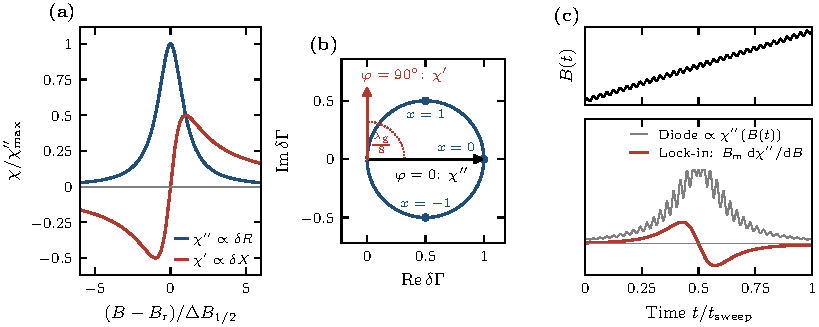
\includegraphics[width=\textwidth]{figures/theory.pdf}
  \caption{Calculated curves (no measurements) for the preparatory exercises. (a)~Absorption $\chiII$ and dispersion
  $\chiI$ of a Lorentzian line versus field. The cavity changes its resistance by $\delta R\propto\chiII$ and its
  reactance by $\delta X\propto\chiI$ (\cref{eq:rx}). (b)~As the field passes through resonance, the change
  $\delta\Gamma\propto\chiII+\ii\chiI$ of the reflected wave traces a circle ($x=(B-\Br)/\Bhalf$). The diode sees only
  its projection onto the reference phase $\varphi$. With $\varphi=0$ it sees absorption, with $\varphi=\ang{90}$
  dispersion. The two settings are a plunger travel of $\lamg/8$ apart. (c)~Field with modulation (top), diode signal
  and lock-in output (bottom), here with $\Bm=\Bhalf/4$ and, for clarity, only 34 modulation periods per sweep.}
  \label{fig:theory}
\end{figure}

\paragraph{Cavity.}
The sample sits in the rectangular cavity (mode TE$_{102}$) where the magnetic microwave field $B_1$ is maximal.
The cavity stores the microwave energy over many oscillations, which enhances the field at the sample. Its
quality factor $\QL\approx930$ corresponds to a resonance width of only $\nu/\QL\approx\qty{10}{MHz}$. Near resonance
the cavity behaves like a series resonant circuit. The sample fills a fraction $\eta$ (filling factor) of the magnetic
field volume and changes the circuit inductance to $L=L_0(1+\eta\chi)$. With
$\chi=\chiI-\ii\chiII$ and the time dependence $e^{\ii\omega t}$ the impedance becomes
\begin{equation}\label{eq:rx}
  Z=R+\ii\omega L_0(1+\eta\chi)+\frac{1}{\ii\omega C}
  \quad\Longrightarrow\quad
  \delta R=\omega L_0\eta\,\chiII,\qquad \delta X=\omega L_0\eta\,\chiI .
\end{equation}

\begin{exercise}{1}
$\chiII$ is a positive Lorentzian with its maximum at resonance (\cref{fig:theory}a). $\chiI$ is positive on one
side of the resonance and negative on the other. It has its extrema at $x=\pm1$, i.e., $\Bhalf$ away from the center,
and further out it falls off only slowly ($\propto1/x$). Since the prefactor $\omega L_0\eta$ is constant during the
field sweep, $\delta R$ follows the absorption exactly and $\delta X$ the dispersion. The sample takes energy from the
cavity, making it lossier, and slightly detunes it. Sweeping the frequency instead of the field gives
exactly the same curves, with $x=(\omega-\omega_0)T_2$.
\end{exercise}

\paragraph{Bridge.}
The signal is the wave reflected by the cavity. If the cavity is coupled so that nothing is reflected at resonance
(critical coupling), the sample produces a small reflected wave
\begin{equation}\label{eq:dgamma}
  \delta\Gamma=\eta\QL\,\bigl(\chiII+\ii\chiI\bigr):
\end{equation}
absorption changes it in phase and dispersion \ang{90} out of phase (\cref{fig:theory}b). On its own this wave
would hardly be measurable, because the diode measures power, $|\delta\Gamma|^2$, the square of a tiny quantity.
A magic T, a waveguide junction with four arms, therefore mixes in a reference wave. The
wave from the source splits between the cavity arm and a reference arm with the attenuator X382A and a movable
short circuit (the \enquote{plunger}). The waves returning from both meet in the fourth arm, where the diode
sits. With $E_c$ the amplitude of the wave at the cavity and $E_be^{\ii\varphi}$ the reference wave at the diode, the
diode measures
\begin{equation}\label{eq:diode}
  V_D\propto\bigl|E_be^{\ii\varphi}+E_c\,\delta\Gamma\bigr|^2
  \approx E_b^2+2E_bE_c\,\eta\QL\bigl(\chiII\cos\varphi+\chiI\sin\varphi\bigr).
\end{equation}
The reference makes the signal linear in $\chi$ and amplifies it by the factor $E_b$. Its phase $\varphi$ selects
absorption, dispersion or a mixture of the two.

\paragraph{Waveguide and plunger.}
The microwave travels in a rectangular waveguide of width $a$. The fundamental mode propagates only if half a
wavelength fits across the width, that is, above the cutoff frequency $\nu_\mathrm c=c/2a$. Above cutoff the wave zigzags
between the walls, and its wavelength along the guide is longer than in free space ($\lambda_0=c/\nu$):
\begin{equation}\label{eq:lamg_theory}
  \lamg=\frac{\lambda_0}{\sqrt{1-(\nu_\mathrm c/\nu)^2}} .
\end{equation}
Moving the plunger by $\Delta z$ lengthens the path of the reference wave by $2\Delta z$, so its phase turns by
$|\Delta\varphi|=4\pi\Delta z/\lamg$.

\begin{exercise}{2}
For $\varphi=0$ the bridge measures $\chiII$ (absorption), for $\varphi=\pm\ang{90}$ it measures $\chiI$ (dispersion).
Switching between them takes a phase change of \ang{90}, so the plunger has to move by $\Delta z=\lamg/8$. For the WR-90
waveguide ($a=\qty{22.86}{mm}$, $\nu_\mathrm c=\qty{6.557}{GHz}$) at $\nu=\qty{9.359}{GHz}$ this gives
$\lamg=\qty{44.89}{mm}$ and $\Delta z=\qty{5.61}{mm}$.
\end{exercise}

\subsection{Field modulation and lock-in}\label{sec:modulation}

The spins change the diode voltage only slightly compared with its bias $E_b^2$, which drifts slowly and
is noisy. So a small modulation $\Bm\cos\omega_\mathrm m t$ with
$\omega_\mathrm m/2\pi=\qty{133}{Hz}$ is added to the field. The diode signal follows the modulation only near
resonance, and the lock-in picks out exactly this part. It multiplies the signal by a reference of the same
frequency and averages over many periods (time constant $\tau$). The output is
$V_\text{out}=\frac12V_sV_r\cos(\psi_r-\psi_s)$, with amplitude $V_s$ and phase $\psi_s$ of the signal and $V_r$, $\psi_r$
of the reference. Everything at other frequencies, including drift and noise, averages out.

\begin{exercise}{3}
$B(t)$ is a slow ramp with a small ripple (\cref{fig:theory}c, top). The diode signal follows
$\chiII(B(t))$, the slowly swept absorption profile with a ripple on top. The ripple amplitude is
proportional to the slope $|\dd\chiII/\dd B|$. On the rising edge the ripple is in phase with the modulation, on the
falling edge in antiphase, and at the line center it vanishes. The lock-in measures its amplitude and sign.
For $\Bm$ small compared with the line width this is
\begin{equation}\label{eq:harmonic}
  V_1(B)\approx\Bm\,\frac{\dd V_D}{\dd B}\propto\Bm\,\frac{\dd\chiII}{\dd B},
\end{equation}
the derivative of the absorption line (\cref{fig:theory}c, bottom). This is why the recorded line shows one positive
and one negative excursion with a zero crossing in the middle instead of a maximum.
\end{exercise}

The extrema of the derivative Lorentzian lie at $\Br\pm\Bhalf/\sqrt3$. Their separation, the peak-to-peak width,
gives $T_2$ directly:
\begin{equation}\label{eq:t2}
  \Bpp=\frac{2}{\sqrt3}\,\Bhalf
  \qquad\Longrightarrow\qquad
  T_2=\frac{2}{\sqrt3\,\gamma\,\Bpp}.
\end{equation}
A larger $\Bm$ gives a larger signal, but only while $\Bm$ is small compared with the line. Once $\Bm$ is comparable to
$\Bpp$, the lock-in averages the derivative over the interval $\pm\Bm$. The measured line gets broader, and the signal
grows more slowly than $\Bm$ (overmodulation). For a Lorentzian, the line is \qty{1}{\percent} too broad at
$\Bm=\Bpp/10$ and already \qty{11}{\percent} too broad at $\Bm=\Bpp/3$. The lab manual therefore recommends $\Bm$
between one fifth and one third of the line width. The sweep must also be slow enough for the low-pass filter of the lock-in
to follow. By a rule of thumb, crossing the line should take at least $10\tau$~\cite{shiroka}.

% ====================================================================
\section{Setup and procedure}\label{sec:setup}
% ====================================================================

\begin{figure}[t]
  \centering
  \resizebox{\textwidth}{!}{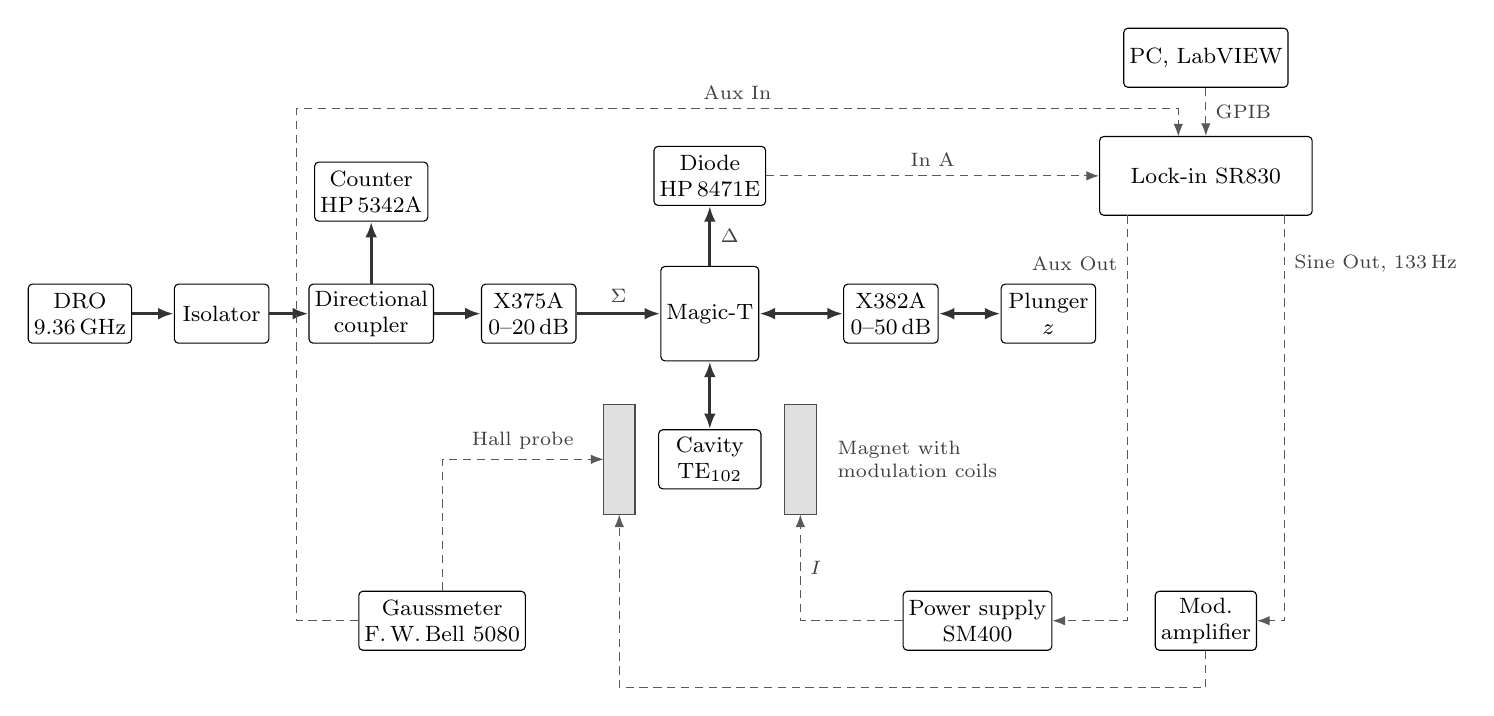
\begin{tikzpicture}[
  font=\footnotesize,
  box/.style={draw, rounded corners=1.5pt, minimum height=7.5mm, minimum width=12mm, align=center, fill=white, inner sep=2pt},
  mw/.style={-{Latex[length=2mm]}, line width=1.1pt, draw=black!80},
  mwb/.style={{Latex[length=2mm]}-{Latex[length=2mm]}, line width=1.1pt, draw=black!80},
  lf/.style={-{Latex[length=1.6mm]}, densely dashed, draw=black!65},
  lbl/.style={font=\scriptsize, text=black!75}]
  % ---------------- Microwave bridge
  \node[box] (dro)  at (-8.0,0) {DRO\\\SI{9.36}{GHz}};
  \node[box] (iso)  at (-6.2,0) {Isolator};
  \node[box] (pick) at (-4.3,0) {Directional\\coupler};
  \node[box] (att1) at (-2.3,0) {X375A\\0--20\,dB};
  \node[box, minimum width=12mm, minimum height=12mm] (tee) at (0,0) {Magic-T};
  \node[box] (att2) at (2.3,0) {X382A\\0--50\,dB};
  \node[box] (plunger) at (4.3,0) {Plunger\\$z$};
  \node[box] (counter) at (-4.3,1.55) {Counter\\HP\,5342A};
  \node[box] (diode) at (0,1.75) {Diode\\HP\,8471E};
  \node[box, minimum width=13mm] (cav) at (0,-1.85) {Cavity\\TE$_{102}$};
  \fill[black!12, draw=black!70] (-1.35,-2.55) rectangle (-0.95,-1.15);
  \fill[black!12, draw=black!70] ( 0.95,-2.55) rectangle ( 1.35,-1.15);
  \node[lbl, align=left, anchor=west] at (1.5,-1.85) {Magnet with\\modulation coils};
  \draw[mw] (dro) -- (iso);
  \draw[mw] (iso) -- (pick);
  \draw[mw] (pick) -- (att1);
  \draw[mw] (pick) -- (counter);
  \draw[mw] (att1) -- node[above, lbl] {$\Sigma$} (tee);
  \draw[mwb] (tee) -- (att2);
  \draw[mwb] (att2) -- (plunger);
  \draw[mwb] (tee) -- (cav);
  \draw[mw] (tee) -- node[right, lbl] {$\Delta$} (diode);
  % ---------------- Electronics
  \node[box, minimum width=27mm, minimum height=10mm] (lockin) at (6.3,1.75) {Lock-in SR830};
  \node[box] (pc) at (6.3,3.25) {PC, LabVIEW};
  \node[box] (delta) at (3.4,-3.9) {Power supply\\SM400};
  \node[box] (modamp) at (6.3,-3.9) {Mod.\\amplifier};
  \node[box] (gauss) at (-3.4,-3.9) {Gaussmeter\\F.\,W.\,Bell 5080};
  \draw[lf] (diode) -- node[above, lbl, pos=0.5] {In A} (lockin.west |- diode);
  \draw[lf] (pc) -- node[right, lbl] {GPIB} (lockin);
  \draw[lf] (5.3,1.25) -- node[pos=0.12, left, lbl] {Aux Out} (5.3,-3.9) -- (delta.east);
  \draw[lf] (7.3,1.25) -- node[pos=0.12, right, lbl] {Sine Out, \SI{133}{Hz}} (7.3,-3.9) -- (modamp.east);
  \draw[lf] (delta.west) -| node[pos=0.75, right, lbl] {$I$} (1.15,-2.55);
  \draw[lf] (modamp.south) |- (0,-4.75) -| (-1.15,-2.55);
  \draw[lf] (gauss.north) |- node[pos=0.75, above, lbl] {Hall probe} (-1.35,-1.85);
  \draw[lf] (gauss.west) -| (-5.25,2.6) -| node[pos=0.25, above, lbl] {Aux In} (5.95,2.25);
\end{tikzpicture}
}
  \caption{X-band reflection spectrometer, drawn with the arms of the magic T as on the real T-piece. Microwave path
  (thick): the DRO source feeds the main attenuator X375A through an isolator and a directional coupler (frequency
  counter). Placed \emph{before} the magic T, it attenuates the cavity and reference waves together. The reference arm
  (top, opposite the cavity) with the reference-arm attenuator X382A and the plunger sets the magnitude and phase of the
  reference. The diode sits at the $\Delta$ port (right). Signal and control lines (dashed): the lock-in supplies the
  control voltage $U$ for the magnet power supply (Aux Out, a DAC output) and the modulation (Sine Out, \qty{133}{Hz})
  and reads the Hall probe (Aux In, an ADC input) and the diode (In A).}
  \label{fig:setup}
\end{figure}

\paragraph{Microwaves.}
\Cref{fig:setup} shows the setup, and \cref{tab:settings} lists all instrument settings. The source is a tunable
dielectric resonator oscillator (DRO, $\geq\qty{13}{dBm}$, i.e.\ at least \qty{20}{mW}). A directional coupler sends
part of its power to the frequency counter. The empty cavity (TE$_{102}$) resonates at \qty{9.3875}{GHz} with a
width of \qty{10.1}{MHz} (network analyzer), so $\QL\approx930$. After every sample change I set X375A to strong
attenuation (\qty{20}{dB}) and retuned the source to the \enquote{dip}, the minimum of the diode voltage where the
cavity absorbs the power. Then I set X375A to \qty{2}{dB}, X382A to \qtyrange{0}{1}{dB} and the plunger to
\qty{20.00}{mm}. With a sample, the resonance was at \qty{9.3594}{GHz} (DPPH) or \qty{9.3527}{GHz} (\ce{MnCl2}). The
detector diode (HP\,8471E) sits at the difference port ($\Delta$) of the magic T.

\paragraph{Fields.}
The electromagnet runs on a current-regulated power supply whose set point is the control voltage
$U=\qtyrange{0}{8}{V}$ from the lock-in. At the DPPH resonance the current is \qty{0.43}{A}. The lock-in's Sine Out
(\qty{133}{Hz}) drives the modulation coils via an amplifier. A gaussmeter (F.\,W.\,Bell\,5080) measures the field
with a Hall probe. I recorded its analog output (\qty{1}{V} corresponds to \qty{1}{T}) and read its display directly. A LabVIEW
program sweeps $U$ in small steps and stores the lock-in outputs $X$ and $Y$ at each step. I set the lock-in phase so
that practically the whole signal lies in $X$ ($Y/X=\num{-0.05}$), and I analyze this component as $S=-X$. I set the
phase with Auto Phase at
$U=\qty{5.9}{V}$, on the high-field flank of the \ce{MnCl2} line (\cref{tab:settings}). There the derivative of the
absorption is negative, but Auto Phase makes the signal positive, so the lock-in phase is \ang{180} off the usual
convention and the raw $X$ has the opposite sign. All fits, figures and signed amplitudes therefore refer to $S=-X$. With it, the derivative of an
absorption line is positive on the rising (low-field) side and negative on the falling (high-field) side, as in
\cref{fig:theory}c.

\paragraph{Measurement program.}
\Cref{tab:scans} lists the analyzed measurements. Before each DPPH scan I set $U$ from \qty{0}{V} to the start value
and held it for \qtyrange{30}{60}{s}. A typical sweep ran at \qty{0.48}{mV/s} of control voltage. To make this independent of the equipment, I convert it
with the slope $\dd B/\dd U=\qty{60.76}{mT/V}$ at the DPPH line (\cref{eq:fieldscale}) and the coil current of
\qty{0.43}{A} at $U=\qty{4.95}{V}$, i.e., \qty{87}{mA/V} if the current is proportional to the set point. The field
then rose at \qty{29}{\micro T/s} (\qty{0.29}{G/s}) and the coil current at about
\qty{42}{\micro A/s}. The DPPH line ($\Bpp=\qty{0.24}{mT}$, \qty{4}{mV} of control voltage) was crossed in about
\qty{8}{s}. This is $27\tau$ for the lock-in time constant $\tau=\qty{300}{ms}$ (the averaging time of its low-pass
filter) and satisfies the rule of thumb from \cref{sec:modulation}. \Cref{tab:scans} gives the field rate of every
scan. These rates use the static slope; during a sweep the field lags behind the set value (\cref{sec:field}), so the
actual rate may be up to \qty{22}{\percent} lower. The DPPH sample is a large
volume of powder. I left out the cut-off scans 07 and 17 (repeated as 07b and 17b) and the first point of every file,
where the signal had not settled. The DPPH search scan 06 overloaded the lock-in, so I only use its zero
crossing, noted in my lab notebook (\cref{sec:mncl2}).

\begin{table}[t]
  \centering\footnotesize
  \caption{Analyzed measurements (23 Oct 2026). $v$: sweep rate of the control voltage; $\dot B$: the corresponding
  field rate $v\,\dd B/\dd U$ with the static slope at the line (\qty{60.76}{mT/V} for DPPH, \qty{61.1}{mT/V} for
  \ce{MnCl2} and \ce{Cu^2+}; for 01--03 the mean slope over the full range). Mod.: Sine Out modulation
  voltage, in parentheses the effective value after amplifier limiting (\cref{sec:modamp}). Attenuators
  main attenuator X375A (cavity and reference) and reference-arm attenuator X382A (reference only) in dB. Sens.: lock-in sensitivity (full scale) in \si{\micro V}.}
  \label{tab:scans}
  \setlength{\tabcolsep}{2.6pt}
  \begin{tabularx}{\textwidth}{@{}l l l l S[table-format=-2.2] S[table-format=-4.0] l c c c >{\raggedright\arraybackslash}X@{}}
    \toprule
    No. & Time & Sample & $U$ (V) & {$v$ (\si{mV/s})} & {$\dot B$ (\si{\micro T/s})} & Mod.\ (V) & X375A & X382A & Sens. & Purpose \\
    \midrule
    01--03 & 10:00 & empty & \numrange{0.10}{8.05} & 25 & 1500 & -- & -- & -- & -- & Hall probe up/down/up \\
    22 & 11:41 & \ce{MnCl2} & \numrange{2.00}{7.98} & 2.86 & 175 & 4 (1.8) & 2 & 1 & 2 & \ce{MnCl2} \\
    07b, 08 & 13:33 & DPPH & \numrange{4.84}{5.13} & 0.95 & 58 & 3; 2 (1.8) & 2 & 1 & 200 & modulation \\
    09--12 & 13:56 & DPPH & \numrange{4.90}{5.01} & 0.48 & 29 & 1--0.1 & 2 & 1 & 200--10 & modulation \\
    13--17b & 14:27 & DPPH & \numrange{4.91}{4.99} & 0.48 & 29 & 1 & 2 & 0--20 & 100--20 & reference arm \\
    18 & 15:14 & DPPH & \numrange{4.99}{4.91} & -0.48 & -29 & 1 & 2 & 6 & 50 & down-sweep \\
    24--27 & 15:24 & DPPH & \numrange{4.91}{4.99} & 0.48 & 29 & 1 & 6--20 & 0 & 100--5 & power series \\
    20 & 15:55 & DPPH & \numrange{4.91}{4.99} & 0.48 & 29 & 1 & 2 & 0 & 200 & dispersion, plunger \qty{25.60}{mm} \\
    19 & 16:05 & -- & \numrange{4.90}{5.00} & & & -- & -- & -- & -- & gaussmeter display at sample \\
    29 & 16:58 & \ce{Cu^2+} & \numrange{4.40}{5.19} & 4.76 & 292 & 4 (1.8) & 2 & 0 & 2 & search \\
    \bottomrule
  \end{tabularx}
\end{table}

\begin{table}[t]
  \centering\footnotesize
  \caption{Instrument settings. Values that vary between scans are in \cref{tab:scans}.}
  \label{tab:settings}
  \begin{tabularx}{\textwidth}{@{}>{\raggedright\arraybackslash}p{0.25\textwidth} >{\raggedright\arraybackslash}X@{}}
    \toprule
    Instrument & Setting \\
    \midrule
    Microwave source & Tunable dielectric resonator oscillator (DRO), $\geq\qty{13}{dBm}$; tuned to the cavity dip after
      every sample change, with X375A at \qty{20}{dB} while tuning \\
    Frequency counter & Via a directional coupler: \qty{9.3594}{GHz} (DPPH), \qty{9.3527}{GHz} (\ce{MnCl2}),
      \qty{9.199}{GHz} (\ce{Cu^2+}, detuned) \\
    Cavity & Rectangular, TE$_{102}$; empty: resonance \qty{9.3875}{GHz}, width \qty{10.1}{MHz} ($\QL\approx930$) \\
    Attenuator X375A (main) & \qty{2}{dB}; \qtyrange{6}{20}{dB} in the power series 24--27 \\
    Attenuator X382A (reference arm) & \qty{1}{dB} (scans 07b--12, 22) or \qty{0}{dB} (13, 20, 24--29); \qtyrange{0}{20}{dB}
      in 13--17b \\
    Plunger (reference arm) & \qty{20.00}{mm} (absorption); \qty{25.60}{mm} (dispersion, scan 20) \\
    Detector & Diode HP\,8471E at the $\Delta$ port of the magic T, connected to lock-in input A and, via a T-piece, to an
      oscilloscope \\
    Lock-in amplifier & Stanford Research SR830, internal reference \qty{133}{Hz}; time constant \qty{300}{ms}
      (\qty{1}{s} in scan 22), filter slope \qty{12}{dB/oct}, reserve Low Noise; phase set once with Auto Phase at
      $U=\qty{5.9}{V}$ before scan 22 and left unchanged afterwards; sensitivity in \cref{tab:scans} \\
    Field modulation & SR830 Sine Out, \qtyrange{0.1}{4}{V} (rms), drives the modulation coils via an amplifier, which
      limits above about \qty{1.8}{V} \\
    Magnet power supply & Delta SM400, current-controlled; set point $U=\qtyrange{0}{8}{V}$ from SR830 Aux Out (DAC);
      \qty{0.43}{A} at the DPPH line \\
    Gaussmeter & F.\,W.\,Bell 5080 with Hall probe (ranges \qtylist{30;300;3000}{mT}, bandwidth dc to
      \qty{20}{kHz}~\cite{fwbell}), range setting \enquote{0.000\,T}; analog output (\qty{1}{V}
      corresponds to \qty{1}{T}) recorded via SR830 Aux In (ADC), display read directly \\
    Field sweep (LabVIEW program EPR\_1) & DPPH: steps of \qty{1}{mV} (\qty{2}{mV} in 07b, 08), \qty{2.1}{s} per point;
      \ce{MnCl2} (22): steps of \qty{20}{mV}, \qty{7}{s} per point; before each scan $U$ set from \qty{0}{V} to the start
      value and held for \qtyrange{30}{60}{s}; back to \qty{0}{V} after each scan \\
    Hall-probe scans 01--03 & LabVIEW program Main\_Field\_Calibration\_2: from \qty{0.1}{V} in 158 steps of \qty{50}{mV},
      \qty{1}{s} wait per step, probe reading averaged over $20\times\qty{50}{ms}$ \\
    \bottomrule
  \end{tabularx}
\end{table}

% ====================================================================
\section{Results and analysis}\label{sec:results}
% ====================================================================
All numbers in this report come from the analysis script \texttt{analysis/analysis.py} in the repository linked on the
title page, which also contains the raw data. Uncertainties are standard deviations ($1\sigma$). I fitted all lines by
nonlinear least squares with a linear baseline; \cref{app:errors} explains the uncertainties.

% --------------------------------------------------------------------
\subsection{Frequency and reference field}\label{sec:frequency}
During the DPPH measurements the frequency counter showed on average $\nu=\qty{9.359378}{GHz}$ (twelve readings, scatter
\qty{22}{kHz}), so the frequency is known far better than any field. For \ce{MnCl2} it was $\nu=\qty{9.352713}{GHz}$.
With the literature value $g_\text{DPPH}=\num{2.0036(2)}$~\cite{poole1996}, \cref{eq:resonance} puts the DPPH resonance at
\begin{equation}\label{eq:bdpph}
  B_\text{DPPH}=\qty{333.75(3)}{mT}.
\end{equation}

% --------------------------------------------------------------------
\subsection{Magnetic field: hysteresis and calibration}\label{sec:field}

\begin{figure}[t]
  \centering
  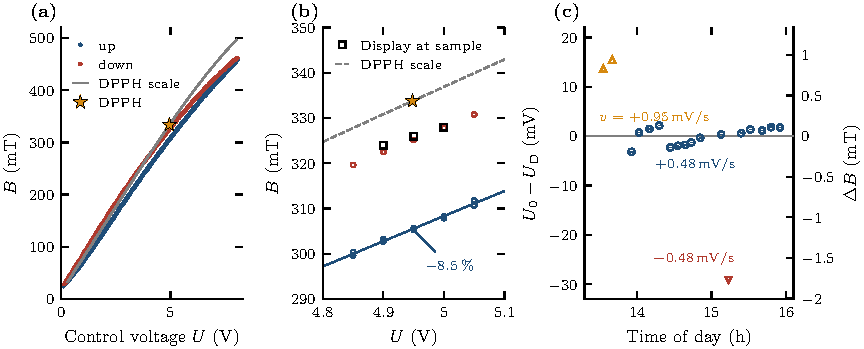
\includegraphics[width=\textwidth]{figures/field.pdf}
  \caption{Main field. (a)~Hall probe (analog output) over the full range: upward (01, 03) and downward (02); in gray the
  field scale calibrated with DPPH (\cref{eq:fieldscale}). (b)~Close-up around the DPPH line: analog output, display at the
  sample position (measurement 19) and the DPPH field (star). The analog output lies \qty{8.5}{\percent}, the display
  \qty{2.3}{\percent} below the DPPH field. (c)~Position $U_0$ of the DPPH line in all scans relative to the mean
  $U_\text{D}$ of the eleven reference scans; triangles: earlier start and doubled sweep rate (orange), down-sweep (red).}
  \label{fig:field}
\end{figure}

\paragraph{Hysteresis.}
Without a sample, I swept the field over the full range up (01, 03) and down (02) (\cref{fig:field}a). Between
\qty{1}{V} and \qty{5.5}{V} the down-sweep lies \qtyrange{14}{24}{mT} above the up-sweeps, and at \qty{0}{V} a residual
field of \qtyrange{17}{24}{mT} remains. I attribute this to hysteresis of the iron yoke: the power supply sets the coil current
via $U$, but the field in the gap also depends on how the iron was magnetized before. For the calibration I use
only up-sweeps, which all start at \qty{0}{V}. Above \qty{0.3}{V} both are described by a cubic polynomial
$B_\text{Hall}(U)$ (scatter \qty{1.1}{mT}).

\paragraph{Calibration.}
In the eleven reference scans (09 to 15 and 24 to 27: jump from \qty{0}{V} to \qtyrange{4.895}{4.910}{V}, wait
\qty{60}{s}, then \qty{0.48}{mV/s}) the DPPH line, more precisely its position $U_0$ in \cref{eq:convolution}, lies on average
at $U_\text{D}=\qty{4.9480}{V}$ (scatter \qty{1.9}{mV}). There the analog output reads \qty{305.4}{mT}, and the display,
read with the probe tip at the center of the cavity, \qty{326}{mT} (\cref{fig:field}b). As $g$-factors these would be
\num{2.189} and \num{2.052} instead of \num{2.0036}. The Hall probe reads too low, the analog output by
\qty{8.5}{\percent} and the display by \qty{2.3}{\percent}.

These are two separate effects. Over the whole range the analog output lies about \qty{6}{\percent} below the display of
the same probe. The probe position would change both readings equally, so the analog output has a scale error of its
own. The remaining \qty{2.3}{\percent} of the display may come from the probe position. According to the course
supervisor (private communication), the gaussmeter is new and may be slightly miscalibrated, and a reading that is too
low usually means that the sensor is not at the height and orientation of maximum reading. A tilt of only \ang{12}
would already explain \qty{2.3}{\percent} ($\cos\ang{12}=\num{0.978}$). The data cannot tell whether the probe sat at its
maximum. I therefore use the gaussmeter only for the \emph{shape} of $B(U)$ and take the scale from DPPH:
\begin{equation}\label{eq:fieldscale}
  B(U)=k\,B_\text{Hall}(U),\qquad k=\frac{B_\text{DPPH}}{B_\text{Hall}(U_\text{D})}=\num{1.0927},
  \qquad \frac{\dd B}{\dd U}\Big|_{U_\text{D}}=\qty{60.76}{mT/V}.
\end{equation}
With this calibration $g_\text{DPPH}$ is no longer measured but sets the scale. I determine the $g$-factor of \ce{MnCl2}
relative to DPPH, so the scale error of the probe cancels. Widths are converted from volts to millitesla with the slope
$\dd B/\dd U$.

\paragraph{The field lags behind.}
With the same protocol the line position is very reproducible. In the eleven scans starting at \qty{4.910}{V} it scatters
by only \qty{0.27}{mV} once a slow drift is removed (\cref{fig:field}c). When the protocol changes, the line jumps. If
the scan starts \qty{75}{mV} earlier (07b, 08), the line lies \qty{19}{mV} higher; in down-sweep~18 it lies \qty{29}{mV}
lower. Ordinary hysteresis cannot explain the first jump, because these scans also start at \qty{0}{V} and run on the
same rising branch. The field lags behind the set value, probably because of a magnetic after-effect in the iron yoke:
it catches up during the wait and falls behind again once the sweep continues. The lag is \qty{22(3)}{\percent} of the
distance swept since the wait and stops growing after a few hundred millivolts (\cref{sec:mncl2}).

This has two consequences. The calibration \cref{eq:fieldscale} only holds for scans run the same way, so the \ce{MnCl2}
scan needs its own reference (\cref{sec:mncl2}). And during the slow scans the field probably rises more slowly than the
static slope says. Since I convert widths with the static slope, they could be up to \qty{22}{\percent} too large. I treat
this as a one-sided systematic.

% --------------------------------------------------------------------
\subsection{DPPH: line width and \texorpdfstring{$T_2$}{T2}}\label{sec:dpph}

\begin{figure}[t]
  \centering
  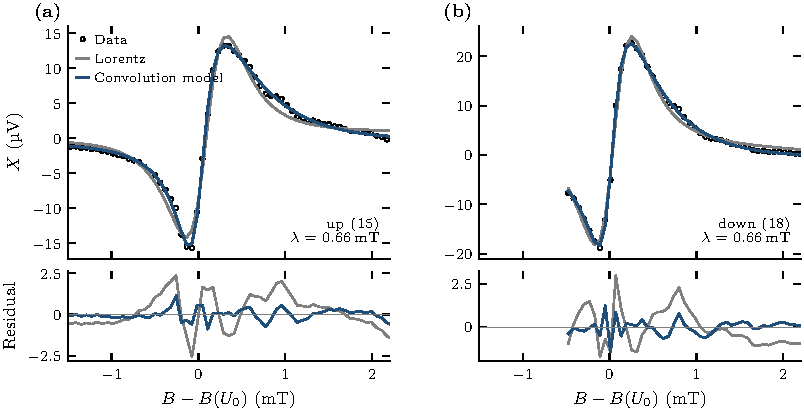
\includegraphics[width=\textwidth]{figures/lineshape.pdf}
  \caption{DPPH line in up-sweep 15 and in down-sweep 18 (otherwise identical settings), shown as the signal $S=-X$
  (\cref{sec:setup}): the derivative of the absorption is positive on the rising and negative on the falling side. Gray: Lorentzian line; blue:
  Lorentzian line convolved with a one-sided field distribution of length $\lambda$ (\cref{eq:convolution}). Bottom: the
  residuals (measurement minus fit). The long tail lies on the high-field side in both sweep directions.}
  \label{fig:lineshape}
\end{figure}

\paragraph{Line shape.}
All DPPH scans show the derivative absorption line from \cref{sec:modulation}, but slightly asymmetric: the flank toward
high field is flatter and longer (\cref{fig:lineshape}). A Lorentzian fits the center but leaves systematic residuals,
and a Gaussian is worse (1.8 times larger residuals). I suspect that the asymmetry comes from field inhomogeneity
across the relatively large powder sample. Parts of the sample would then reach resonance at slightly higher coil
currents, which gives a tail toward high field. To account for this, I fitted a Lorentzian convolved with a one-sided
exponential field distribution of length $\lambda$:
\begin{equation}\label{eq:convolution}
  S(U)=\int_0^\infty\frac{\dd u}{\lambda}\,e^{-u/\lambda}\,
  \frac{\dd}{\dd x}\biggl[\frac{a}{1+x^2}+\frac{d\,x}{1+x^2}\biggr]_{x=(U-U_0-u)/G}+b_0+b_1U .
\end{equation}
Here $U_0$ is the line position without the tail and $G$ the HWHM of the Lorentzian in units of the control voltage. The
amplitudes $a$ and $d$ belong to absorption and dispersion; a small dispersion part is needed because the bridge phase is
never exactly zero. The baseline is $b_0+b_1U$. This model reduces the residuals by a factor of 3. The length
$\lambda=\qty{13.5(5)}{mV}$ corresponds to \qty{0.82}{mT}, or \qty{0.25}{\percent} of the field. Down-sweep~18 supports
this explanation over the field lag: a lag would move the tail to the other side when sweeping down, but the tail stays
on the same side with the same length. \Cref{tab:dpphfits} in \cref{app:fits} lists the fit results
of every DPPH scan.

\paragraph{Width and \texorpdfstring{$T_2$}{T2}.}
The data do not show what the field distribution looks like at its edge. Other distributions (gamma, half-Cauchy) fit
just as well but give a $G$ up to \qty{10}{\percent} smaller. I take the middle of this range, $G=\qty{3.43}{mV}$, and
with \cref{eq:t2} and the slope from \cref{eq:fieldscale} obtain
\begin{equation}\label{eq:t2dpph}
  \Bpp=\frac{2}{\sqrt3}\,G\,\frac{\dd B}{\dd U}=\qty{0.240(15)}{mT},\qquad
  T_2=\frac{2}{\sqrt3\,\gamma\,\Bpp}=\qty{27(2)}{ns}.
\end{equation}
Most of the uncertainty comes from this choice of model (half the range, \qty{0.013}{mT}); field scale
(\qty{0.007}{mT}) and statistics (\qty{0.003}{mT}) contribute less. If the field rises more slowly during the scan than
assumed (\cref{sec:field}), the line is up to \qty{22}{\percent} narrower and $T_2$ up to \qty{35}{ns} long. A bound
without any model also exists. The simple Lorentzian fit assigns the whole field distribution to the line and gives
$\Bpp=\qty{0.51}{mT}$. Since the distribution can only broaden the line, $T_2\geq\qty{12.8}{ns}$. Reported values for
DPPH are \qtyrange{0.15}{0.47}{mT}~\cite{poole1996}, depending on crystal form and included solvent; my value lies in
this range.

This measurement cannot give the $g$-factor of DPPH independently, because DPPH is the calibration. With the display of
the Hall probe alone I would have obtained $g=\num{2.052}$, \qty{2.4}{\percent} above the literature value. This matches
the \qty{2.3}{\percent} by which the display reads too low.

% --------------------------------------------------------------------
\subsection{Modulation amplitude}\label{sec:modamp}

\begin{figure}[t]
  \centering
  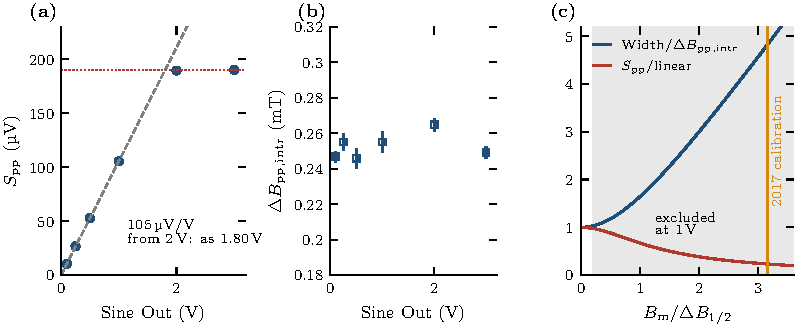
\includegraphics[width=\textwidth]{figures/modulation.pdf}
  \caption{Modulation series (scans 07b to 12). (a)~Peak-to-peak signal versus the Sine Out voltage: proportional up to
  \qty{1}{V}; from \qty{2}{V} on, the amplifier limits. (b)~Width of the Lorentzian line in the convolution model:
  independent of the modulation. (c)~Calculated width and amplitude of the first harmonic of a pure Lorentzian line versus
  $\Bm/\Bhalf$. Gray: excluded at \qty{1}{V} for a pure Lorentzian line (for the measured profile the limit lies slightly
  higher, \cref{eq:bm}); orange: what the 2017 calibration would give at \qty{1}{V}.}
  \label{fig:modulation}
\end{figure}

I tried to measure the alternating field of the modulation coils directly with the gaussmeter in AC mode, at the
modulation frequency of \qty{133}{Hz} and on its most sensitive range, \qty{30}{mT} (\qty{300}{G}, resolution
\qty{10}{\micro T}). The F.\,W.\,Bell 5080 has no lower range, and its bandwidth (dc to \qty{20}{kHz}) covers
\qty{133}{Hz}~\cite{fwbell}. At all Sine Out voltages (\qtyrange{0.1}{4}{V}) it showed only its noise
(\qty{0.04}{mT}). The limit was therefore the sensitivity, not the frequency: the bound derived below,
$\Bm<\qty{0.06}{mT}$ at \qty{1}{V} and $<\qty{0.11}{mT}$ in the limited state, is comparable to this noise. A very
low modulation frequency (e.g.\ \qty{0.1}{Hz}) would have let me follow the oscillating field in DC mode and average
over many periods; I did not try this. Such a calibration would still have to be transferred to \qty{133}{Hz}, because
the inductive impedance of the modulation coils grows with frequency. Since the direct measurement failed, the DPPH
lines themselves give an upper bound on $\Bm$.

In the modulation series I changed only the Sine Out voltage $U_\mathrm m$ (\cref{fig:modulation}). Up to \qty{1}{V} the
peak-to-peak signal $S_\mathrm{pp}$ (the distance between maximum and minimum of the line) grows in proportion to
$U_\mathrm m$ (\qty{105.4}{\micro V/V}, scatter about \qty{1}{\percent}), as \cref{eq:harmonic} requires for small
$\Bm$. At \qty{2}{V} and \qty{3}{V} the signal is the same, \qty{190}{\micro V}: the modulation amplifier limits, and
both settings act like \qty{1.80}{V}. The width does not change; the ratio of the widths in the limited state and at
\qtyrange{0.1}{1}{V} is \num{1.025(36)}.

This is what bounds $\Bm$. In the limited state the signal, and with it $\Bm$, is 1.8 times as large as at \qty{1}{V},
yet the line is not wider. \Cref{fig:modulation}c shows how a line broadens as $\Bm$ grows. For the width ratio to stay
below its upper $2\sigma$ limit of \num{1.096}, the measured line profile requires
\begin{equation}\label{eq:bm}
  \Bm(\qty{1}{V})<\qty{0.059}{mT},\qquad \Bm(\text{limited})<\qty{0.11}{mT}.
\end{equation}
At \qty{1}{V}, the setting of all other DPPH scans, $\Bm$ is at most a quarter of $\Bpp$ and broadens the
fitted line by at most \qty{3}{\percent}. A previous report on this setup gives the 2017 calibration
$\Bm=\qty{5.06}{G/V}\cdot U_\mathrm m+\qty{1.8}{G}$. At \qty{1}{V} this would be \qty{0.69}{mT}, almost three times
$\Bpp$. The line would then be 2.8 times wider at \qty{1}{V} than at \qty{0.1}{V}, and the signal would grow by only a
factor of 1.1 in between. I measured equal widths (ratio \num{1.03(3)}) and a factor of 10.1, so the old calibration does
not hold for the present setup.

\paragraph{Effect of the modulation amplitude.}
As long as $\Bm$ is small compared with the line width, the signal grows in proportion to $\Bm$ and the line shape stays
the same. A large $\Bm$ gives a good signal-to-noise ratio, a small one an undistorted width; the lab manual recommends
one fifth to one third of the line width. For DPPH, $\Bm$ at \qty{1}{V} was at most a quarter of $\Bpp$, so within or
below this range, and the amplifier could not reach overmodulation. For \ce{MnCl2}, $\Bm$ is at least a thousand times
smaller than the line, because the resonance is very broad. The signal becomes tiny (\cref{sec:mncl2}), but the line shape stays exact.

% --------------------------------------------------------------------
\subsection{Microwave power and reference arm}\label{sec:power}

\begin{figure}[t]
  \centering
  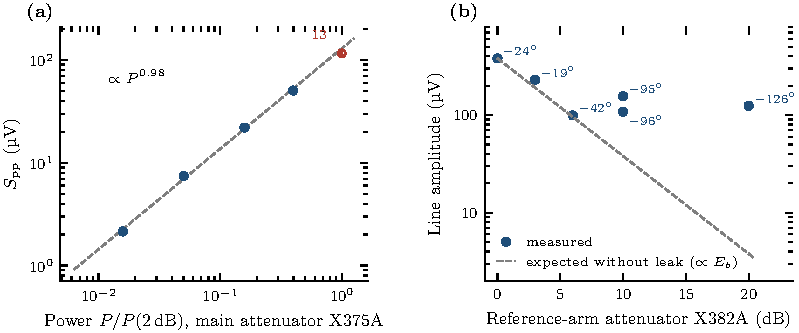
\includegraphics[width=\textwidth]{figures/power.pdf}
  \caption{Role of the two attenuators. The main attenuator X375A sits before the magic T and sets the microwave power
  at the cavity (and the reference with it). The reference-arm attenuator X382A only weakens the reference wave and
  leaves the power at the cavity unchanged. (a)~Power series with the main attenuator X375A (scans 24 to 27 at
  \qtyrange{6}{20}{dB}, scan 13 at \qty{2}{dB}):
  peak-to-peak signal versus power relative to \qty{2}{dB}; dashed: the fit to 24 to 27. Scan~13 (red)
  comes from an earlier measurement block. (b)~Series with the reference-arm attenuator X382A (scans 13 to 17b):
  magnitude of the line, $|a+\ii d|$ from \cref{eq:convolution}, and its phase $\arg(a+\ii d)$ (for the signal $S=-X$). Dashed: the decrease if the
  signal were proportional to the reference amplitude, which passes through X382A twice.}
  \label{fig:power}
\end{figure}

\paragraph{Power series.}
The main attenuator X375A sits before the magic T. It attenuates the wave to the cavity and the reference wave equally, so both amplitudes
grow with $\sqrt P$. By \cref{eq:diode} a square-law diode then gives a signal proportional to $E_bE_c\propto P$; a
detector measuring the amplitude instead of the power would give only $\sqrt P$. Over \qty{14}{dB} I find
$S_\mathrm{pp}\propto P^{\num{0.98(3)}}$ (\cref{fig:power}a). This is consistent with square-law detection, and I
found no sign of saturation over the investigated power range.

Saturation is not expected either. At most a few milliwatts reach the cavity, so the microwave field at the sample is
only $B_1\approx\qtyrange{3}{6}{\micro T}$. With $T_1\approx T_2=\qty{27}{ns}$ (plausible for an exchange-narrowed
radical) the saturation parameter $s=\gamma^2B_1^2T_1T_2$ is below \num{1e-3}; noticeable saturation would need more than
\qty{1}{W}. Scan~13 lies \qty{10}{\percent} below the straight line, but its line shape argues against saturation as well.
Saturation would reduce the absorption more than the dispersion. In scan~13 it is the other way round: the absorption
part is \qty{86}{\percent} of the mean of scans 24 to 27 (scatter \qty{8}{\percent}), the dispersion part only
\qty{52}{\percent} (scatter \qty{9}{\percent}). Since mainly dispersion is missing, I look for the cause in the bridge rather than in the spins (below).

\paragraph{Series with X382A.}
In scans 13 to 17b I changed the reference-arm attenuator X382A instead. It leaves the power at the cavity unchanged and only
weakens the reference wave $E_b$ in \cref{eq:diode}. The reference passes through it twice, so at \qty{20}{dB} $E_b$
drops by a factor of 100, and the signal $\propto E_b$ should drop by the same factor (dashed in \cref{fig:power}b).
In fact its magnitude drops only by a factor of 3.1, and its phase rotates by \ang{-102}, from mostly absorption to
mostly dispersion. I explain this with a \enquote{leak}: the cavity is not perfectly matched and itself sends a small
wave to the diode, of about a quarter of the reference amplitude. The weaker the reference, the more the leak takes over its role, and its
phase, not that of the plunger, decides which part of $\chi$ the diode sees. The signal is largest without attenuation
of the reference (\qty{0}{dB}). Only X375A is suitable for power series.

\paragraph{Size of the leak.}
I estimated the size of the leak from two independent measurements. With the leak $\rho e^{\ii\psi}$ added to the reference amplitude
$r=10^{-A/10}$ ($A$ is the X382A setting, passed twice), \cref{eq:diode} requires each part of the signal to be linear
in $r$. The absorption part is: $a=\alpha r+\beta$ with $\alpha=\qty{589}{\micro V}$ and $\beta=\qty{-73}{\micro V}$,
scatter \qty{6}{\micro V} for $r=\numrange{0.01}{0.5}$. The offset $\beta$ is the leak, and at $A=\qty{9.1}{dB}$ reference
and leak cancel in the absorption. The dispersion part is not reproducible. Scans 16 and 16b, taken with the same
settings, have the same absorption part (\qty{-12.3}{\micro V} and \qty{-12.0}{\micro V}) but dispersion parts of
\qty{-156}{\micro V} and \qty{-108}{\micro V}. The leak seems to drift, mainly in the dispersion, which is also the part
missing in scan~13.

The second measurement is the DC voltage of the diode at zero field, which I read on the oscilloscope for seven settings
of X382A between \qty{0}{dB} and \qty{20}{dB}. Without a line the diode sees only reference and leak,
$V_D=z-V_0\,|r+\rho e^{\ii\psi}|^2$, with the oscilloscope zero $z$ (the voltage is negative). The readings follow this
with $V_0=\qty{2.92(10)}{mV}$ and $\rho\cos\psi=\num{-0.204}$, scatter \qty{0.019}{mV}; for a single pass through X382A
the scatter would be five times larger. I did not measure $z$, but it must be at least the largest reading,
\qty{0.351}{mV}, so $\rho\geq\num{0.20}$. With $z=\qty{0.42}{mV}$, which also fits the line sizes of 13 to 17b,
$\rho=\num{0.26}$ and $\cos\psi=\num{-0.78}$. The leak is a quarter of the reference and partly cancels it: the diode
bias drops from \qty{1.93}{mV} at \qty{0}{dB} to \qty{0.08}{mV} at \qty{6.9}{dB}. Above about \qty{7}{dB} the leak is the
stronger wave, which is why the line turns into dispersion at \qtyrange{10}{20}{dB}.

The absorption part of scan~13 is also off the straight line (\qty{348}{\micro V} instead of \qty{516}{\micro V}).
Scaled to \qty{2}{dB}, scans 13 and 24 to 27 reach on average only 0.76 of the line value, as if \qty{1.2(4)}{dB} less
power had reached the cavity than in 14 to 18. At 15:53 I wrote in my lab notebook that I might have set X375A to
\qty{1}{dB} instead of \qty{2}{dB} before. Such a step between the blocks would explain the difference. I compare
signal sizes and phases only within one block; positions, widths and line shapes are not affected.

% --------------------------------------------------------------------
\subsection{Dispersion and guide wavelength}\label{sec:dispersion}

\begin{figure}[t]
  \centering
  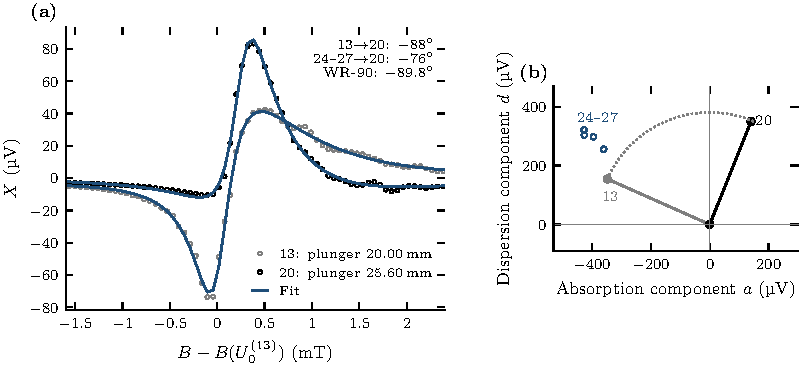
\includegraphics[width=\textwidth]{figures/dispersion.pdf}
  \caption{Dispersion. (a)~Scan~13 (plunger at \qty{20.00}{mm}) and scan~20 (\qty{25.60}{mm}), otherwise identical
  settings, shown as the signal $S=-X$, with fits according to \cref{eq:convolution}. The angles at the top right are the measured phase rotations and the
  value for WR-90. (b)~Complex amplitudes $a+\ii d$ of the lines: 13, 20 and 24 to 27 (same plunger position as 13,
  scaled to the same power); dotted: the rotation by the WR-90 value.}
  \label{fig:dispersion}
\end{figure}

For scan~20 I moved only the plunger, from \qty{20.00}{mm} (scan~13) to \qty{25.60}{mm}. This is
$\Delta z=\qty{5.60}{mm}$, almost exactly $\lamg/8$, i.e., $\lamg/4$ in the path of the reference wave (preparatory exercise~2). The line with a zero crossing at the center
becomes a line with a minimum at the center and two shallow side maxima (\cref{fig:dispersion}a): $\dd\chiII/\dd B$ turns
into $-\dd\chiI/\dd B$, as expected for a bridge phase rotated by \ang{-90} (\cref{eq:diode}).

To quantify this, I combine the absorption part $a$ and the dispersion part $d$ of each line (\cref{eq:convolution}) into the
complex amplitude $a+\ii d$. Its angle is the effective bridge phase $\varphi$ in \cref{eq:diode}: the phase of the
total reference wave at the diode, to which the leak from the cavity (\cref{sec:power}) contributes besides the
reference arm. The plunger rotates it by
\ang{-87.9} and leaves the magnitude unchanged (ratio \num{0.99}, \cref{fig:dispersion}b). Repeated scans at a fixed
plunger position scatter in phase by only \ang{1.1}, but the starting angle is uncertain. Scans 24 to 27, taken at the
same plunger position as 13 and shortly before scan~20, lie \ang{12} away from scan~13 because the leak drifts. With this
difference as a systematic uncertainty, $\Delta\varphi=\qty{-88(13)}{\degree}$, and $|\Delta\varphi|=4\pi\Delta z/\lamg$
together with \cref{eq:lamg_theory} gives
\begin{equation}\label{eq:lamg}
  \lamg=\frac{\ang{720}\,\Delta z}{|\Delta\varphi|}=46^{+8}_{-6}\,\unit{mm},\qquad
  \nu_\mathrm c=\nu\sqrt{1-(\lambda_0/\lamg)^2}=6.7^{+0.8}_{-1.1}\,\unit{GHz}.
\end{equation}
Despite the large uncertainty, the result is consistent with the WR-90 waveguide ($\lamg=\qty{44.9}{mm}$,
$\nu_\mathrm c=\qty{6.56}{GHz}$), and $\lamg$ is clearly larger than the free-space wavelength
$\lambda_0=\qty{32.0}{mm}$, which would correspond to \ang{-126}. The plunger displacement of \qty{5.60}{mm} also agrees
with the $\lamg/8$ needed to switch between absorption and dispersion.

\paragraph{Check without a line model.}
Absorption and dispersion are not independent. Because of causality (the spins cannot respond before they are driven),
$\chiI$ and $\chiII$ are Hilbert transforms of each other (Kramers--Kronig relations). The Hilbert transform $H$ commutes with the
derivative and with the smearing by the field distribution. The measured line $S_{13}$ and its transform $H[S_{13}]$ must
therefore give the line at any other bridge phase, whatever its exact shape:
\begin{equation}\label{eq:hilbert}
  S_{20}(U)=k\bigl[\cos D\,S_{13}+\sin D\,H[S_{13}]\bigr](U-\delta U)+b_0+b_1U .
\end{equation}
I computed $H[S_{13}]$ numerically from the data, with the fitted curve supplying the tails outside the scan window. The
fit gives $D=\qty{-84.3(7)}{\degree}$ and $k=\num{0.98}$. Its residuals (\qty{1.43}{\micro V}) are as small as those of
the free fit of scan~20 with \cref{eq:convolution} (\qty{1.41}{\micro V}). Within the noise, the two measured lines
therefore behave as a Kramers--Kronig pair, and the rotation angle follows without an assumption on the line shape. It
agrees with the \ang{-87.9} of the model fits within the systematic uncertainty. Starting from scans 24 to 26 instead of
13 gives \ang{-75} to \ang{-77}, an offset of about \ang{10}, like the one the drifting leak causes above.

% --------------------------------------------------------------------
\subsection{\texorpdfstring{\ce{MnCl2}}{MnCl2}: an exchange-narrowed line}\label{sec:mncl2}

\begin{figure}[t]
  \centering
  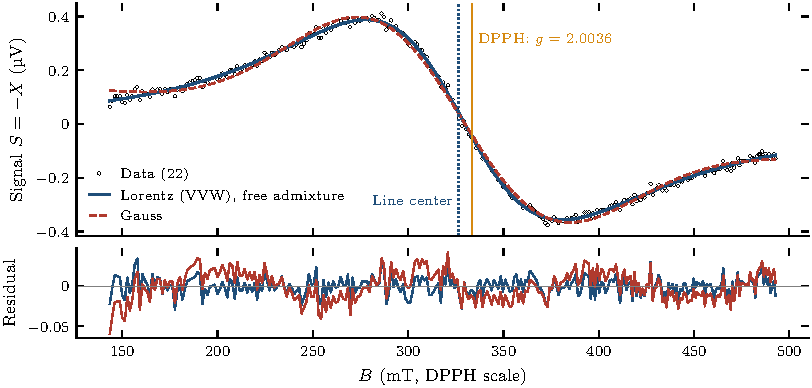
\includegraphics[width=\textwidth]{figures/mncl2.pdf}
  \caption{\ce{MnCl2}, scan~22 on the field scale with the reference \cref{eq:udmn}, shown as the signal $S=-X$. Blue: Lorentzian line according to
  \cref{eq:vvw} with free dispersion admixture and linear baseline; red dashed: Gaussian line. Bottom: the residuals.
  Vertical lines: line center (dotted) and the position that $g=\num{2.0036}$ would have at this frequency.}
  \label{fig:mncl2}
\end{figure}

\paragraph{Line shape and width.}
Scan~22 covers \qtyrange{143}{493}{mT} and shows a single line with $\Bpp\approx\qty{103}{mT}$ (\cref{fig:mncl2}); none
of the six hyperfine lines of \ce{^{55}Mn} is visible. The signal is small, \qty{0.74}{\micro V}, although \ce{MnCl2}
has a 76 times larger static susceptibility than DPPH, because the derivative of a line more than 400 times wider is
correspondingly flat. A Lorentzian describes the data within the noise (residuals \qty{1.5}{\percent} of the signal,
without visible structure). A Gaussian fits 1.6 times worse and misses the data on both flanks. A Lorentzian line is
what exchange narrowing predicts (\cref{sec:width}).

Because the line is so broad ($\Bhalf\approx0.27\,\Br$), a detail matters that plays no role for DPPH. Besides the
co-rotating component, the linearly polarized microwave field also has a counter-rotating one. It is resonant at
$B=-\Br$, and the tail of this second line reaches into the measurement window. The absorption is therefore
\begin{equation}\label{eq:vvw}
  \chiII(B)\propto\frac{1}{1+\Bigl(\frac{B-\Br}{\Bhalf}\Bigr)^2}+\frac{1}{1+\Bigl(\frac{B+\Br}{\Bhalf}\Bigr)^2}.
\end{equation}
Since the line is almost as wide as the measurement window, its position depends somewhat on the fit window and the
baseline: $g$ lies between \num{2.045} and \num{2.060}. Without the dispersion admixture I would get
$g=\numrange{2.028}{2.034}$, but that fit is clearly worse in every window I tried. The width is robust:
\begin{equation}\label{eq:mnwidth}
  \Bhalf=\qty{88.8(23)}{mT},\qquad T_2=\frac{1}{\gamma\Bhalf}=\qty{62(2)}{ps}.
\end{equation}
Without exchange, the dipolar fields of the neighbors would give a Gaussian line with an HWHM of about \qty{250}{mT}
(\cref{sec:width}). The measured line is a third as wide and Lorentzian. By \cref{eq:aw} this requires an exchange field
$B_\text{ex}\approx\qtyrange{0.5}{0.7}{T}$, comparable to the resonance field itself.

\paragraph{Field reference.}
For $g$, what matters is the field at which the scan passed the line center (\qty{4.854}{V}). The reference
$U_\text{D}$ from \cref{eq:fieldscale} does not apply, because scan~22 reached the line only after a run-up of
\qty{2.9}{V}, while the DPPH reference scans had a run-up of only \qty{38}{mV} (\cref{sec:field}). I take the
reference from the DPPH scans with a long run-up. Scans 07b and 08 (\qty{128}{mV} run-up) give \qty{4.9626}{V}, and the
DPPH search scan~06 (\qty{383}{mV}) gives \qty{4.983}{V}. They differ by only \qty{20}{mV} despite three times the
run-up, so the field lag stops growing after a few hundred millivolts. I assume that the reference of scan~22 lies
between these two values. Taking this bracket as a uniform distribution and adding the reading uncertainty and the drift
gives
\begin{equation}\label{eq:udmn}
  U_\text{D}^{(22)}=\qty{4.973(12)}{V}.
\end{equation}

\paragraph{\texorpdfstring{$g$}{g}-factor.}
Relative to this reference (\cref{eq:grel}),
\begin{equation}\label{eq:gmn}
  g\bigl(\text{\ce{MnCl2}}\bigr)=\num{2.058(11)} .
\end{equation}
The uncertainty comes mainly from the line shape (fit window and baseline, \num{0.008}), from the sample in the cavity
(\num{0.005}) and from the field reference (\num{0.005}). The sample detunes the cavity slightly, sees a field that is
not quite homogeneous, like DPPH, and shifts the field inside it with its own magnetization. Statistics, field scale and
$g_\text{DPPH}$ together contribute \num{0.003} (\cref{app:errors}). A gap in my lab notebook leaves a one-sided
systematic. Before scan~22 I set the field to \qty{5.9}{V} to adjust the lock-in phase, and I did not write down whether
I brought it back to \qty{0}{V} afterwards. If not, the scan ran on a different branch of the hysteresis curve, and $g$
would be smaller by up to \num{0.025}.

The line width lets me test this. On the other branch the field would rise more slowly across the line, because the gap
to the normal branch shrinks from \qty{5.6}{mT} at \qty{4.2}{V} to \qty{1.6}{mT} at \qty{5.6}{V} (estimated from the
hysteresis loop in \cref{fig:field}a). Scan~22 would then look 1.054 times wider than the search scan I recorded just
before, which did start from \qty{0}{V} (\qtyrange{2.00}{7.95}{V} at \qty{50}{mV/s}; signal in $Y$, because I set the
lock-in phase only afterwards). A joint fit of both scans, each part weighted by its own scatter, gives a width ratio of
\num{0.963(39)}. This is $2.3\sigma$ below the prediction for the other branch and $0.9\sigma$ below the normal branch.
The test favors the normal branch but cannot rule out the other one, on which $g=\num{2.032(11)}$.

\paragraph{Origin of \texorpdfstring{$g>2$}{g > 2}.}
For \ce{Mn^2+} without orbital moment one expects $g=\numrange{2.000}{2.002}$~\cite{abragam1970}; the measured value is
\num{0.057(11)} higher. I do not think this is an error of the field scale. A more likely explanation is the large width itself. The dipolar
coupling between the spins does not only broaden the line; it also contains terms that flip spins at the frequencies $\omega_0$
and $2\omega_0$. For narrow lines they average out, but for a line as wide as a quarter of the resonance field they shift
the resonance to higher frequency, that is, to lower field at fixed frequency, and $g$ appears larger. From the measured
width and without a free parameter, the theory of Kubo and Tomita~\cite{kubo1954} predicts $\Delta g=\numrange{0.028}{0.055}$,
which is consistent with the measurement.

% --------------------------------------------------------------------
\subsection{\texorpdfstring{\ce{Cu^2+}}{Cu2+}: no usable result}\label{sec:cu}
Scan~29 on the copper sample shows only noise (\qty{0.021}{\micro V}) and no line. This says nothing about \ce{Cu^2+},
however. In the repeat scan with the same settings the frequency counter showed \qty{9.199}{GHz}, about \qty{160}{MHz}
below the cavity resonance; when retuning I had not found a real dip. This far from resonance the signal is about 1000
times smaller. The noise of the scan still shows how sensitive it would have been on the dip: a single Lorentzian line
with $\Bpp=\qty{10}{mT}$ would have shown up ($3\sigma$) with only \qty{13}{\percent} of the number of spins in the DPPH
sample (\qty{3}{\percent} for \qty{5}{mT}, about as many as in DPPH for \qty{30}{mT}). The scan covered
$g=\numrange{1.89}{2.19}$. The measurement has to be repeated with a properly tuned source.

% ====================================================================
\section{Discussion}\label{sec:discussion}
% ====================================================================
\begin{table}[t]
  \centering\small
  \caption{Results at a glance ($1\sigma$; one-sided systematics in parentheses).}
  \label{tab:results}
  \begin{tabularx}{\textwidth}{@{}l l >{\raggedright\arraybackslash}X@{}}
    \toprule
    Quantity & Result & Comparison \\
    \midrule
    Hall probe at sample position & \qty{-8.5}{\percent} (analog), \qty{-2.3}{\percent} (display) & DPPH as standard \\
    Hysteresis of the yoke & \qtyrange{14}{24}{mT}, residual field \qtyrange{17}{24}{mT} & -- \\
    DPPH: $g$ with display & \num{2.052} & \num{2.0036}~\cite{poole1996} \\
    DPPH: $\Bpp$, $T_2$ & \qty{0.240(15)}{mT}, \qty{27(2)}{ns} (up to \qty{35}{ns}) & \qtyrange{0.15}{0.47}{mT}~\cite{poole1996} \\
    Modulation at \qty{1}{V} & $\Bm<\qty{0.059}{mT}$ & recommended: $\Bpp/5$ to $\Bpp/3$ \\
    Power dependence & $S_\mathrm{pp}\propto P^{\num{0.98(3)}}$ & square-law diode: $P^1$ \\
    Bridge leak & $\rho\approx\num{0.26}$, $\cos\psi\approx\num{-0.78}$ & -- \\
    Dispersion, model-free & $D=\qty{-84.3(7)}{\degree}$ & model fit: \ang{-87.9} \\
    Guide wavelength & $\lamg=46^{+8}_{-6}\,\unit{mm}$ & WR-90: \qty{44.9}{mm} \\
    Cutoff frequency & $\nu_\mathrm c=6.7^{+0.8}_{-1.1}\,\unit{GHz}$ & WR-90: \qty{6.56}{GHz} \\
    \ce{MnCl2}: $\Bhalf$, $T_2$ & \qty{88.8(23)}{mT}, \qty{62(2)}{ps} & without exchange: about \qty{250}{mT} \\
    \ce{MnCl2}: $g$ & \num{2.058(11)} (\num{-0.025}) & $\num{2.001}+\Delta g$, $\Delta g=\numrange{0.028}{0.055}$ \\
    \bottomrule
  \end{tabularx}
\end{table}

\paragraph{Magnetic field.}
The magnetic-field calibration was the largest source of uncertainty in this experiment (\cref{tab:results} collects
all results). At the sample position the Hall probe reads too low, and only the DPPH calibration turns the control voltage into a
reliable field. Next time I would first move the probe to the height and orientation with the highest reading, as the
course supervisor recommends. Any deficit left after that would point to the gaussmeter calibration. The DPPH
calibration holds only for scans run exactly like the DPPH scans. Because the field lags behind the set point, starting
just \qty{75}{mV} earlier shifts the line by \qty{1.2}{mT}, almost five times the DPPH line width. This
causes the three large systematics of the report: the DPPH width may be overestimated by up to \qty{22}{\percent}, the
field reference for \ce{MnCl2} is uncertain, and the \ce{MnCl2} scan may have run on a different hysteresis branch. A
small marker sample would avoid all three, for example a grain of DPPH next to the sample in the cavity. It would appear
in every scan, with the same magnetic history as the measurement. Without a marker, every scan should start from
\qty{0}{V} with the same dwell time and sweep rate, and every deviation should be noted in the lab notebook.

\paragraph{Modulation and DPPH.}
For the modulation amplitude I only have an upper bound. A small pick-up coil at the sample position would have measured
it directly. According to the course supervisor (private communication), such a coil is available in the lab, in the
drawer with the waveguide parts; I did not ask for it during the measurement: with 100 turns on \qty{10}{mm^2} and $\Bm=\qty{0.05}{mT}$ it would give about \qty{40}{\micro V}, easy to
measure with the lock-in. The value of $T_2$ rests on the convolution model, because the large powder sample sees a
field distribution of \qty{0.82}{mT}, almost four times the HWHM of the line. With only a few grains in the center of the
cavity, a plain Lorentzian fit would give $T_2$ directly.

\paragraph{Bridge.}
The lab manual uses the main attenuator for the power dependence and the attenuator in the reference arm for
balancing the bridge, and my measurements support this choice. With X375A the signal follows the power linearly, as
expected for a diode at low power, while X382A changes only the reference. The Hilbert-transform fit shows without any
line model that absorption and dispersion obey the Kramers--Kronig relations within the noise. The leak of
the cavity makes phases comparable only within one measurement block and limits the accuracy of $\lamg$ to about
\qty{15}{\percent}. Several plunger positions in quick succession would give a more accurate value. The complex amplitude
then moves on a circle around the fixed leak contribution, and the rotation angle per millimeter can be fitted
independently of it.

\paragraph{\texorpdfstring{\ce{MnCl2}}{MnCl2} and copper.}
The \ce{MnCl2} line shows the typical features of exchange narrowing. It is Lorentzian, has no hyperfine structure, and is
only a third as wide as the dipolar fields would make it without exchange. If the deviation of its $g$-factor from 2 comes
from the large width, as I suspect, it should almost vanish at higher frequency. The copper measurement has to be repeated
with a properly tuned source, reading the frequency from the counter before and after each scan.


\appendix
% ====================================================================
\section{Error analysis}\label{app:errors}
% ====================================================================

\paragraph{Fits.}
I fitted all lines by least squares with equal weights (\texttt{curve\_fit} from SciPy). The exception is the joint
fit of the two \ce{MnCl2} scans in \cref{sec:mncl2}, where I weighted each scan, and each part of the search scan,
by the inverse of its own residual scatter. I scaled the covariance matrix with the residual variance
$s^2=\sum_ir_i^2/(N-n_\mathrm p)$ ($N$ data points, $n_\mathrm p$ fit parameters), so that the uncertainties reflect
the actual scatter. For averages over several scans I took the larger of the internal and external uncertainty:
\begin{equation}\label{eq:wmean}
  \bar x=\frac{\sum_jw_jx_j}{\sum_jw_j},\qquad w_j=\sigma_j^{-2},\qquad
  \sigma_{\bar x}=\max\!\left[\Bigl(\sum_jw_j\Bigr)^{-1/2},\ \frac{s_x}{\sqrt n}\right],
\end{equation}
where $s_x$ is the standard deviation of the $n$ individual values.

\paragraph{Reference field.}
By \cref{eq:resonance}, $B_\text{DPPH}=h\nu/(g_\text{DPPH}\muB)$, so
\begin{equation}
  \frac{\sigma_B}{B}=\sqrt{\left(\frac{\sigma_g}{g}\right)^2+\left(\frac{\sigma_\nu}{\nu}\right)^2}
  =\sqrt{(\num{1.0e-4})^2+(\num{2.3e-6})^2}=\num{1.0e-4},
\end{equation}
and $\sigma_B=\qty{0.033}{mT}$. Only the literature value of $g_\text{DPPH}$ counts; the frequency contributes nothing.

\paragraph{Field scale.}
With $B(U)=k\,B_\text{Hall}(U)$ and $k=B_\text{DPPH}/B_\text{Hall}(U_\text{D})$ (\cref{eq:fieldscale}),
\begin{equation}
  \frac{\sigma_k}{k}=\sqrt{\left(\frac{\sigma_{B_\text{DPPH}}}{B_\text{DPPH}}\right)^2
  +\left(\frac{B_\text{Hall}'(U_\text{D})\,\sigma_{U_\text{D}}}{B_\text{Hall}(U_\text{D})}\right)^2}
  =\num{1.4e-4},
\end{equation}
where $\sigma_{U_\text{D}}=\qty{1.9}{mV}/\sqrt{11}$. I converted widths with the slope
$B'=k\,B_\text{Hall}'(U_\text{D})=\qty{60.76}{mT/V}$. Different descriptions of the calibration curve
(polynomial degree, scale or zero-point error of the display) give a slope uncertainty of
$\sigma_{B'}/B'=\qty{3.0}{\percent}$. The field lag (\cref{sec:field}) is not included; it enters as a one-sided
systematic.

\paragraph{Line width and \texorpdfstring{$T_2$}{T2}.}
With $\gamma=g\muB/\hbar$ of the respective sample, $\Bpp=2B'G/\sqrt3$ and $T_2=1/(\gamma B'G)$. Both carry the
relative uncertainties of $G$ and $B'$:
\begin{equation}
  \frac{\sigma_{T_2}}{T_2}=\frac{\sigma_{\Bpp}}{\Bpp}=\sqrt{\left(\frac{\sigma_G}{G}\right)^2+\left(\frac{\sigma_{B'}}{B'}\right)^2}.
\end{equation}
Here $\sigma_G$ includes the fit error and the model uncertainty from \cref{sec:dpph}.

\paragraph{\texorpdfstring{$g$}{g}-factor relative to DPPH.}
For a line at $U_x$ and frequency $\nu_x$,
\begin{equation}\label{eq:grel}
  g_x=\frac{h\nu_x}{\muB\,k\,B_\text{Hall}(U_x)}
  =g_\text{DPPH}\,\frac{\nu_x}{\nu_\text{DPPH}}\,\frac{B_\text{Hall}(U_\text{D})}{B_\text{Hall}(U_x)} .
\end{equation}
The factor $k$ drops out, and with it the scale error of the probe. The remaining uncertainties are those of the
literature value $g_\text{DPPH}$, the reference position $U_\text{D}$ and the line position $U_x$:
\begin{equation}
  \frac{\sigma_{g_x}}{g_x}=\sqrt{\left(\frac{\sigma_{g_\text{DPPH}}}{g_\text{DPPH}}\right)^2
  +\left(\frac{B'_\text{Hall}(U_\text{D})\,\sigma_{U_\text{D}}}{B_\text{Hall}(U_\text{D})}\right)^2
  +\left(\frac{B'_\text{Hall}(U_x)\,\sigma_{U_x}}{B_\text{Hall}(U_x)}\right)^2}.
\end{equation}
For \ce{MnCl2}, $\sigma_{U_\text{D}}=\qty{12}{mV}$ (\cref{eq:udmn}) contributes \num{0.0046} and the fit error of $U_x$
contributes \num{0.0024}. I estimated the other contributions in \cref{sec:mncl2} (line shape \num{0.0076}, sample in
the cavity \num{0.0052}, shape of the calibration curve and $g_\text{DPPH}$ together \num{0.0010}) from how much $g$
changes when I vary the line model, the calibration curve and the corrections. All contributions added in quadrature
give \num{0.0106}.

\paragraph{Guide wavelength.}
The phase rotation $\Delta\varphi$ for the plunger displacement $\Delta z$ gives $\lamg=\ang{720}\,\Delta z/|\Delta\varphi|$
and $\nu_\mathrm c=\nu\sqrt{1-(\lambda_0/\lamg)^2}$ with $\lambda_0=c/\nu$. Error propagation gives
\begin{equation}
  \frac{\sigma_{\lamg}}{\lamg}=\sqrt{\left(\frac{\sigma_{\Delta\varphi}}{\Delta\varphi}\right)^2
  +\left(\frac{\sigma_{\Delta z}}{\Delta z}\right)^2},\qquad
  \sigma_{\nu_\mathrm c}=\frac{c^2}{\nu_\mathrm c\,\lamg^3}\,\sigma_{\lamg} .
\end{equation}
Compared with the phase, the plunger scale (\qty{0.01}{mm}) contributes nothing. Because $\lamg$ is inversely
proportional to $|\Delta\varphi|$, the symmetric interval $\Delta\varphi=\qty{-88(13)}{\degree}$ becomes the asymmetric
interval $\lamg=46^{+8}_{-6}\,\unit{mm}$. I computed its limits directly from $|\Delta\varphi|=\ang{75}$ and \ang{101}.

% ====================================================================
\section{Fit results of the DPPH scans}\label{app:fits}
% ====================================================================
% generated by analysis/tables.py -- do not edit by hand
\begin{center}
  \footnotesize\setlength{\tabcolsep}{3.4pt}\captionsetup{hypcap=false}
  \captionof{table}{Fit results of all analyzed DPPH scans. Convolution model (\cref{eq:convolution}): position $U_0$, intrinsic
  HWHM $G$, length $\lambda$ of the field distribution, mixing angle $\varphi_\ast=\operatorname{atan2}(d,a)$. Simple
  Lorentzian fit: $G_\mathrm{L}$, $\varphi_\mathrm{L}$. Last column: ratio of the residual rms of both fits.
  \qty{1}{mV} corresponds to \qty{60.76}{\micro T}; attenuators in dB; arrow: sweep direction.}
  \label{tab:dpphfits}
  \sisetup{table-number-alignment=center, uncertainty-mode=compact}
  \begin{tabular}{@{}l S[table-format=1.2] S[table-format=2.0] S[table-format=2.0] c S[table-format=3.1] S[table-format=1.4] S[table-format=1.2(2)] S[table-format=2.1(2)] S[table-format=-3.0] S[table-format=1.2] S[table-format=-3.0] S[table-format=1.1]@{}}
    \toprule
    Scan & {Mod.\ (V)} & {X382A} & {X375A} & & {$S_\mathrm{pp}$ (\si{\micro V})} & {$U_0$ (V)} & {$G$ (mV)} & {$\lambda$ (mV)}
      & {$\varphi_\ast$ (\si{\degree})} & {$G_\mathrm{L}$ (mV)} & {$\varphi_\mathrm{L}$ (\si{\degree})} & {$\frac{\mathrm{rms_L}}{\mathrm{rms}_\ast}$} \\
    \midrule
    07b & 3 & 1 & 2 & $\uparrow$ & 190.1 & 4.9617 & 3.55(4) & 15.8(5) & 141 & 7.64 & -172 & 3.3 \\
    08 & 2 & 1 & 2 & $\uparrow$ & 189.4 & 4.9635 & 3.77(5) & 14.1(5) & 143 & 7.76 & -173 & 3.2 \\
    09 & 1 & 1 & 2 & $\uparrow$ & 105.3 & 4.9448 & 3.64(8) & 14.5(10) & 143 & 7.53 & -170 & 3.0 \\
    10 & 0.5 & 1 & 2 & $\uparrow$ & 52.8 & 4.9487 & 3.50(8) & 14.5(9) & 144 & 7.41 & -169 & 2.7 \\
    11 & 0.25 & 1 & 2 & $\uparrow$ & 26.8 & 4.9495 & 3.64(7) & 14.4(7) & 146 & 7.56 & -168 & 3.3 \\
    12 & 0.1 & 1 & 2 & $\uparrow$ & 10.4 & 4.9501 & 3.52(4) & 15.2(7) & 145 & 7.43 & -167 & 3.4 \\
    13 & 1 & 0 & 2 & $\uparrow$ & 115.9 & 4.9457 & 3.94(9) & 12.3(11) & 156 & 7.51 & -160 & 2.3 \\
    14 & 1 & 3 & 2 & $\uparrow$ & 65.3 & 4.9461 & 3.64(9) & 12.3(10) & 161 & 7.03 & -153 & 2.3 \\
    15 & 1 & 6 & 2 & $\uparrow$ & 28.9 & 4.9462 & 3.42(7) & 10.8(7) & 138 & 6.65 & -179 & 3.1 \\
    16 & 1 & 10 & 2 & $\uparrow$ & 39.0 & 4.9467 & 3.49(5) & 12.1(5) & 85 & 7.12 & 131 & 3.9 \\
    16b & 1 & 10 & 2 & $\uparrow$ & 27.9 & 4.9477 & 3.49(5) & 11.4(6) & 84 & 7.00 & 128 & 3.4 \\
    17b & 1 & 20 & 2 & $\uparrow$ & 30.4 & 4.9484 & 3.55(7) & 12.2(7) & 54 & 7.12 & 101 & 3.0 \\
    18 & 1 & 6 & 2 & $\downarrow$ & 41.5 & 4.9188 & 3.17(5) & 10.9(6) & 124 & 6.01 & 180 & 2.4 \\
    24 & 1 & 0 & 6 & $\uparrow$ & 50.4 & 4.9486 & 3.84(9) & 12.8(11) & 145 & 7.37 & -170 & 2.6 \\
    25 & 1 & 0 & 10 & $\uparrow$ & 22.0 & 4.9494 & 3.77(7) & 12.9(10) & 143 & 7.30 & -171 & 2.9 \\
    26 & 1 & 0 & 15 & $\uparrow$ & 7.4 & 4.9491 & 3.75(8) & 12.5(9) & 145 & 7.21 & -170 & 2.9 \\
    27 & 1 & 0 & 20 & $\uparrow$ & 2.1 & 4.9498 & 3.67(5) & 13.8(8) & 143 & 7.25 & -168 & 3.6 \\
    20 & 1 & 0 & 2 & $\uparrow$ & 93.9 & 4.9498 & 4.02(11) & 13.0(9) & 68 & 8.02 & 113 & 2.8 \\
    \bottomrule
  \end{tabular}
\end{center}



\section*{Acknowledgment}
I used the AI model Claude by Anthropic~\cite{claude} for help with the analysis code and the text.

{\small% ====================================================================
\begin{thebibliography}{9}\setlength{\itemsep}{1pt}
\bibitem{shiroka} T.~Shiroka, \emph{Introduction to Electron-Spin Resonance (ESR) Spectroscopy}, lab manual,
  Physics Lab Course, ETH Zürich.
\bibitem{poole1996} C.~P.~Poole, \emph{Electron Spin Resonance: A Comprehensive Treatise on Experimental Techniques},
  2nd~ed., Dover, New York (1996).
\bibitem{vanvleck1948} J.~H.~Van~Vleck, \emph{The dipolar broadening of magnetic resonance lines in crystals},
  Phys.\ Rev.\ \textbf{74}, 1168 (1948).
\bibitem{anderson1953} P.~W.~Anderson, P.~R.~Weiss, \emph{Exchange narrowing in paramagnetic resonance},
  Rev.\ Mod.\ Phys.\ \textbf{25}, 269 (1953).
\bibitem{kubo1954} R.~Kubo, K.~Tomita, \emph{A general theory of magnetic resonance absorption},
  J.\ Phys.\ Soc.\ Jpn.\ \textbf{9}, 888 (1954).
\bibitem{abragam1970} A.~Abragam, B.~Bleaney, \emph{Electron Paramagnetic Resonance of Transition Ions},
  Clarendon Press, Oxford (1970).
\bibitem{claude} Anthropic, \emph{Claude}, AI model, \url{https://www.anthropic.com/claude} (2026).
\end{thebibliography}
}

\end{document}
